\documentclass[preprint]{sigplanconf}
\usepackage{minted}
\usepackage{graphicx}
\usepackage{amsmath}
\usepackage{xcolor}
% The following \documentclass options may be useful:

% preprint      Remove this option only once the paper is in final form.
% 10pt          To set in 10-point type instead of 9-point.
% 11pt          To set in 11-point type instead of 9-point.
% numbers       To obtain numeric citation style instead of author/year.


\definecolor{lbcolor}{rgb}{0.95,0.95,0.95}

\newcommand{\cL}{{\cal L}}

\begin{document}

\special{papersize=8.5in,11in}
\setlength{\pdfpageheight}{\paperheight}
\setlength{\pdfpagewidth}{\paperwidth}

\conferenceinfo{CONF 'yy}{Month d--d, 20yy, City, ST, Country}
\copyrightyear{20yy}
\copyrightdata{978-1-nnnn-nnnn-n/yy/mm}
\copyrightdoi{nnnnnnn.nnnnnnn}

% Uncomment the publication rights you want to use.
%\publicationrights{transferred}
%\publicationrights{licensed}     % this is the default
%\publicationrights{author-pays}

% \titlebanner{banner above paper title}        % These are ignored unless
\preprintfooter{short description of paper}   % 'preprint' option specified.

\title{Polite programmers, write with sentences.}

\authorinfo{Mircea F. Lungu}
           {Software Architecture Group,
           University of Groningen}
           {m.f.lungu@rug.nl}
\authorinfo{Jan Kurs}
           {Software Composition Group,
           University of Bern}
           {kurs@inf.unibe.ch}

\maketitle

\begin{abstract}

\noindent
TheJavaPeopleUseCamelCaseToSeparateWordsInTheirIdentifiers. 

\noindent
Pythonistas\_and\_their\_friends\_use\_underscore\_in\_their\_identifiers. 

\noindent
Polite programmers use sentence case to recall that code is prose.
\end{abstract}
\vspace {1cm}
\category{CR-number}{subcategory}{third-level}

% \keywords
% keyword1, keyword2

%!TEX root=../paper.tex


\section{Introduction}

Polite is an evolution of the Smalltalk programming language that aims to encourage developers to think more about their programs as prose. The main mechanism by which Polite does this is what we define here as sentence case identifiers -- a naming convention that allows spaces in identifier names. Polite illustrates that it is possible to embed spaces in identifier names while still storing and editing programs as text. 

Although spaces in identifiers have been used before in DSLs (e.g. Applescript, the Cucumber testing framework, Inform 7) or COBOL, the feature is unusual for a general purpose object-oriented text-based programming language. We suspect that the main reason for this is historical: spaces allow the scanner to easily tokenize the text in a traditional compiler backend architecture. We believe howevr, that easing the job of the programmer should come before easing the job of the scanner. 

If a syntax like that of Polite will encourage developers to think more about their programs as prose, and thus maybe work just a little bit harder towards writing more beautiful and readable code, it would be worth investigating using sentence case identifiers in other languages. Indeed, since software developers spend the largest part of their time reading code rather than writing it, even the smallest increase in code readability is to be fought for and cherished.
Some readers will argue that nobody in their right mind would use such long identifiers as we illustrated in the abstract. For those readers, we report three method names that can be found in popular open source programs written in one of the most popular programming languages at the moment: 


\begin{minted}[bgcolor=lbcolor]{text}
// nakedobjects-4.0.0
whenCallEnsureThatContextOverloadedShouldThrowIll
egalThreadStateExceptionUsingSuppliedMessage 

// aspectj-1.6.9
getPointcutParserSupportingSpecifiedPrimitivesAnd
UsingSpecifiedClassLoaderForResolution 

// maven-3.0
disabledtestResolveCorrectDependenciesWhenDiffer
entDependenciesOnNewestVersionReplaced 
\end{minted}





%!TEX root=../paper.tex

\section{Illustrating the Polite Syntax}

To experiment with sentence case identifiers, we started from the grammar of Smalltalk and we modified all the rules that involve identifiers to allow spaces in identifier names. Once this was done, we discovered several other grammar modifications which we considerd desirable. We named the resulting language Polite Smalltalk or for short, Polite. Others in the past have also started from Smalltalk and provided deltas to augment its syntax \cite{Born87}.

In this section we discuss those modifications to the original  Smalltalk language that were performed to obtain Polite.

% Polite, the language that we propose here, started as an experiment in evolving the syntax of Smalltalk to using sentence case identifiers. We thus started from the Smalltalk grammar that we had implemented as a parsing expression grammar and iteratively modified it. 

% It is derived from Smalltalk to which we add sentence case identifiers, first class functions, and the concept of a program. 

% The syntax of Polite is basically that of Smalltalk-80, to which we bring several modifications. The reader can thus assume the Smalltalk syntax, and we will discuss the modifications in this section. 

\newcommand{\comma}{{`,' }}
\newcommand{\plus}{{`+' }}
\newcommand{\code}[1]{{\texttt{#1}}}

\subsection{Sentence Case Identifiers}
In Smalltalk, to send to an object a unary message, one simply separates the two with a space, e.g.

\begin{minted}{text} 
politeHero rechargeEnergy.
\end{minted}

Keyword messages are similar but they are separated by their arguments with a column, e.g.

\begin{minted}{text} 
politeHero fightWith: anEnemy.
\end{minted}


If we want to allow spaces in the name of identifiers, we cannot use space to separate the object and the message. 
In Polite we introduce a comma to separate the name of an agent from the message that is receives, as one would also do in natural language (e.g. {\em ``Alfred, get the Batwing ready''}). All the characters in an identifier including the spaces are relevant for its identity. The previous code snippets thus become: 

\begin{minted}{text} 
polite hero, recharge energy. 
polite hero, fight with: an enemy.
\end{minted}

For the seasoned Smalltalkers, using a comma in this way might be anathema since the operator is traditionally used to concatenate strings and other collections. However, such a sentiment is misplaced since comma is just a simple message implemented in the Collection class. In Polite, the \plus operator takes over the responsibilities of \comma and is thus used to concatenate two collections.


\subsection{Polite Programs}
The Smalltalk grammar does not provide productions for programs or classes, since the programmer grows a program by compiling a method at a time in the Smalltalk IDE. 

To be able to write programs independent of the Smalltalk IDE we introduce a new grammar rule for a program: a sequence of class and global method definitions, followed by code to be executed. The following code snippet presents a simple program with one class definition and a few lines of code: 
\vspace{0.5em}

\inputminted[bgcolor=lbcolor,linenos]{text}{polite-hero.polite}

\vspace{0.5em}
In the code snippet we see several other features of the language: 

\begin{itemize}

	\item A class declaration (line 1) has the syntax of a message sent to the superclass for creating the subclass. 

	\item Indentation based scoping is used for defining the body of a class and the body of a method. 

	\item Class, program, and method local variable declarations (lines~2 and 17) are enumerated between pipes and must be separated by~\comma (line 2)

\end{itemize}


\subsection {First Class Functions}
Polite allows the definition of first class functions as opposed to Smalltalk where a method must always be part of a class. These functions are global to the program. 

One of the benefits of this, is the possibility of implementing new control structures like the one used in lines 10--14 from the example program: 

\begin{minted}{text}
while neither: [self, is dead] 
	  nor: [an enemy, is dead] 
	   do: [self, fight with: an enemy] 
\end{minted}

The possibility of defining such ad-hoc control structures, that other languages like Grace or Scala also provide, can be used to improve the readability of program text. This is especially beneficial for several of the conditional structures of Smalltalk which were shown in a study by Stefik to be unintuitive for newcomers to the language \cite{Stef13}. To illustrate the difference in readability, compare the previous code with the equivalent traditional Smalltalk: 

\begin{minted}{text}
((self isDead not) and: [anEnemy isDead not]) 
	whileTrue: [self fightWith: anEnemy]
\end{minted}




% The highlighted line of code will be hard to read for beginners [citation about control structures in St being hard in general for beginners] and could even be error prone for advanced developers.  shows the usefulness of having first class functions. Especially since the control structures of Smalltalk turn out to puzzle beginners [citation needed]. 

%!TEX root=../paper.tex

\section{Implementation}
Polite is implemented on top of Pharo Smalltalk and PetitParser is used to define its grammar using parsing expressions. The implementation can be found online. The code examples from this paper are fragments of a larger example that can also be found in the Polite image available online. 

\begin{figure}[h]
	\centering
	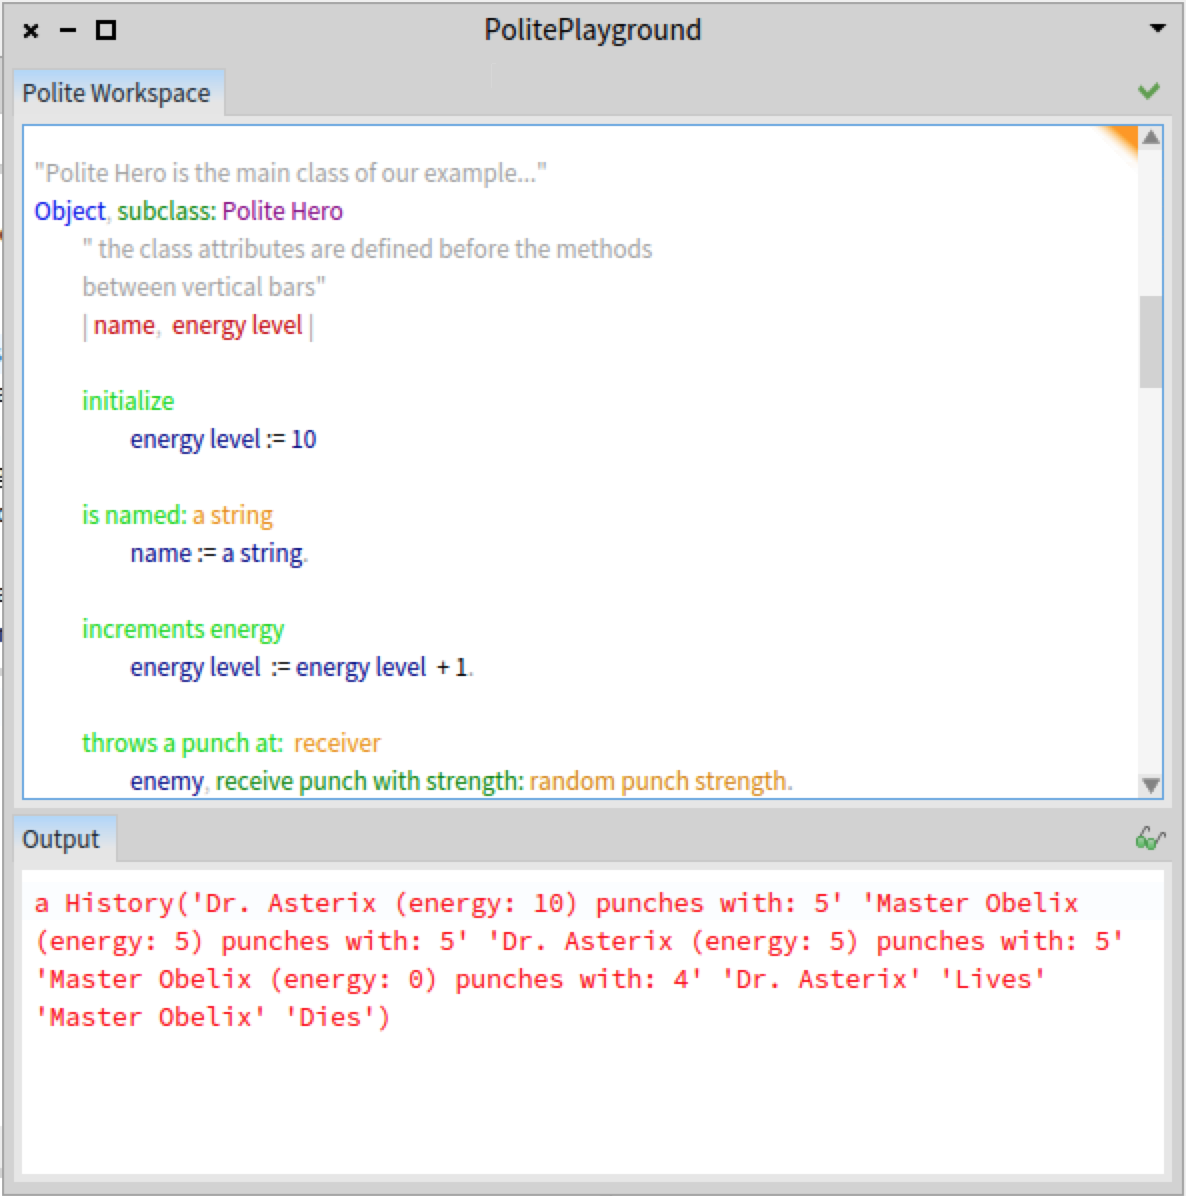
\includegraphics[width=0.45\textwidth]{images/playground.png}
	\caption{The Polite Playground provides a syntax highlighting code editor for Polite}
	\label{fig:figure1}
\end{figure}


\acks

We would like to thank Oscar Nierstrasz and Tijs van der Storm for feedback on earlier versions of this paper.



% We recommend abbrvnat bibliography style.

\bibliographystyle{abbrvnat}
\bibliography{mir-biblio/polite}

% The bibliography should be embedded for final submission.

% \begin{thebibliography}{}
% \softraggedright

% \bibitem[Smith et~al.(2009)Smith, Jones]{smith02}
% P. Q. Smith, and X. Y. Jones. ...reference text...

% \end{thebibliography}


\end{document}
